\documentclass[Softwaredesign/Softwaredesign_main.tex]{subfiles}
\begin{document}
\textbf{Resource list}\\
Under GUI projektet findes en fil "resource\_list"; filen indeholder en liste af \#defines, som definere en masse shorthands for stylesheets. Et stylesheet et tilsvarende for CSS for et HTML objekt, den tilpasser udsenet for et objekt, som f.eks. et Qlabel. alle de her stylesheets bruger stier som føre til forskellige billeder,  som bruges i GUI delen af RPI applikationen.  Dog for at denne liste af stier altid skal være den samme: altså statiske, er der brug for en ".qrc" fil. Dette er en QT resource fil, som kan indeholde prefixes til forskellige formater af filer.  Gennem dette "pic" prefix kan der tilgås en liste af billeder filer;  alle billederne findes i deres egen "pictures folder" inde i projekt mappen. Denne mappe indeholder alle billederne som bruges i GUI'en.  For at se et diagram over relationen for alt det overnævnte henvises til figur \ref{fig:resource_list}.
alt dette leder til at alle stier til billederne nu start med ":pic/pictures". For eksemepl ville stien til "gameboard" billedet være ":pic/pictures/gameboard.png".
\begin{figure}
    \centering
    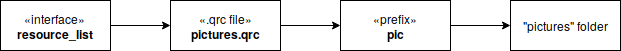
\includegraphics[scale=0.5]{Softwaredesign/GUI/Pictures/resource_list.png}
    \caption{Diagram over brug af resource list}
    \label{fig:resource_list}
\end{figure}
\end{document}




